\documentclass[11pt, parskip=half]{scrartcl}

\usepackage[lithuanian]{azuma}
\usepackage[raggedbottom]{stablespacing}
\usepackage[a4paper, margin=1in]{geometry} % center margins
\usepackage{needspace}
\usepackage{enumitem}
\usepackage{booktabs}
\usepackage{pgfplots}
\pgfplotsset{compat=newest}
\setlist[itemize]{topsep=0pt, itemsep=0.1em} %partopsep, parsep

\begin{document}
    \title{1-as lab. darbas}
    \subtitle{9-as variantas}
    \maketitle

    % ----- PROBLEM 1 -----
    \begin{problem}
        Apskaičiuokite $\sum_{k=10}^{30}\frac{i^k}{1+i}$
    \end{problem}

    \begin{solution}
        \begin{equation}
            \sum_{k=10}^{30}\frac{i^k}{1+i} = \frac{i^{10} + i^{11} + \dots + i^{28} + i^{29} + i^{30}}{1+i} \label{eq:trig}
        \end{equation}
        Žinome, kad:
        \begin{equation}
            i^{4n} + i^{4n+1} + i^{4n+2} + i^{4n+3} = 1 + i + (-1) + (-i) = 0, \quad n \in \mathbb{N}
            \label{eq:complexperiod}
        \end{equation}
        Pritaikom $\pmod{4}$ redukciją visiem laipsniam:
        \begin{equation}
            \frac{i^{10} + i^{11} + \dots + i^{28} + i^{29} + i^{30}}{1+i}
            = \frac{i^2 + i^3 + i^0 + i^1 + i^2 + i^3 + \dots + i^0 + i^1 + i^2}{1 + i}
            \label{eq:4reduced}
        \end{equation}
        Iš ~\eqref{eq:4reduced} ir ~\eqref{eq:complexperiod} išplaukia:
        \[
        \frac{i^2 + i^3 + 0 + \dots + i^0 + i^1 + i^2}{1 + i}
        = \frac{i^2 + i^3 + i^0 + i^1 + i^2}{1 + i}
        = \frac{i^2}{1 + i}
        \]
        \[
        = \frac{-1}{1 + i}
        = \frac{-1(1 - i)}{(1 + i)(1 - i)}
        = \frac{i - 1}{2}
        = -\frac{1}{2} + \frac{1}{2}i
        \]
    \end{solution}
    
    % ----- PROBLEM 2 -----
    \begin{problem}
        Tarkime $u=3+3i, w=2-2i, z=4+2i$, apskaičiuokite $|z| + \bar{u} + \frac{w^2}{|w|}$
    \end{problem}

    \begin{solution}
        \[
        |z| + \bar{u} + \frac{w^2}{|w|}
        = \sqrt{4^2 + 2^2} + 3-3i + \frac{(2-2i)^2}{\sqrt{2^2 + (-2)^2}}
        = \sqrt{20} + 3 - 3i + \frac{-8i}{\sqrt{8}}
        \]
        \[
        = 2\sqrt{5} + 3 - 3i + \frac{-8i}{2\sqrt{2}}
        = 2\sqrt{5} + 3 - 3i - 2\sqrt{2}\,i
        \]
        \[
        = (2\sqrt{5}+3) + (-3-2\sqrt{2})i
        \]
    \end{solution}

    % ----- PROBLEM 3 -----
    \begin{problem}
        Užrašykite $z = - \frac{80}{3} - \frac{80}{3}i$ trigonometrinėje formoje $re^{i \theta}$
    \end{problem}

    \begin{solution}
        \[
            r = |z| = \sqrt{\left(-\frac{80}{3}\right)^2 + \left(-\frac{80}{3}\right)^2}
            = \frac{80\sqrt{2}}{3}
        \]
        \[
            \theta = \arctan \left(\frac{-\frac{80}{3}}{-\frac{80}{3}}\right)
            = \arctan(1) = \frac{\pi}{4}
        \]
        Kadangi $a = - \frac{80}{3}, b = - \frac{80}{3}$ t.y. $a < 0$ ir $b < 0$, $z$ yra 3-iame ketvirtyje, o $\frac{\pi}{4}$
        mums duoda 1-ą ketvirtį, todėl pridedame $\pi$, kad pataisyti:
        \[
        \theta = \frac{\pi}{4} + \pi = \frac{5\pi}{4}
        \]
        Taigi turime:
        \[
        z = - \frac{80}{3} - \frac{80}{3}i = \frac{80\sqrt{2}}{3} e^{i(\frac{5\pi}{4} + 2\pi k)}, k \in \mathbb{Z}
        \]
    \end{solution}

    % ----- PROBLEM 4 -----
    \begin{problem}
        Išspręskite lygtį $3x^2 + 2x + 10 = 0$
    \end{problem}

    \begin{solution}
        \[
            x = \frac{-b \pm \sqrt{b^2 - 4ac}}{2a}
        \]
        Čia $a=3, \; b=2, \; c=10$. Todėl:
        \[
            x = \frac{-2 \pm \sqrt{2^2 - 4\cdot 3 \cdot 10}}{2\cdot 3}
            = \frac{-2 \pm \sqrt{4 - 120}}{6}
        \]
        \[
            = \frac{-2 \pm \sqrt{-116}}{6}
            = \frac{-2 \pm i\sqrt{116}}{6}
        \]
        \[
            = \frac{-2 \pm 2i\sqrt{29}}{6}
            = \frac{-1 \pm i\sqrt{29}}{3}
        \]
        Taigi sprendiniai yra:
        \[
            x_1 = \frac{-1}{3} + \frac{\sqrt{29}}{3}i, 
            \quad 
            x_2 = \frac{-1}{3} - \frac{\sqrt{29}}{3}i
        \]
    \end{solution}

    % ----- PROBLEM 5 -----
    \begin{problem}
        Raskite skaičiaus $z=-1-i$ visas $8$-tąsias šaknis.
    \end{problem}

    \begin{solution}
        \[
            r = |z| = \sqrt{(-1)^2+(-1)^2} = \sqrt{2}, 
            \quad
            \theta = \frac{5\pi}{4}.
        \]
        Todėl:
        \[
            z = \sqrt{2}e^{i(\frac{5\pi}{4})}.
        \]
        Taigi:
        \[
            z_k = 2^{\frac{1}{16}}e^{i(\frac{5\pi}{32} + \frac{k\pi}{4})}, \quad k=0,1,\dots,7.
        \]
    \end{solution}

    % ----- PROBLEM 6 -----
    \begin{problem}
        Nubraižykite sritį kompleksinėje plokštumoje, kurią atitinka visi skaičiai $z$, kurie tenkina sąlygas: $|2z| \leq 5, \quad \arg(z) < \frac{\pi}{3}$
    \end{problem}

    \begin{solution}
        Kadangi $|2z|\le 5$, tai $|z|\le \frac{5}{2}$ ir spindulys $r = \frac{5}{2}$.

        \begin{center}
            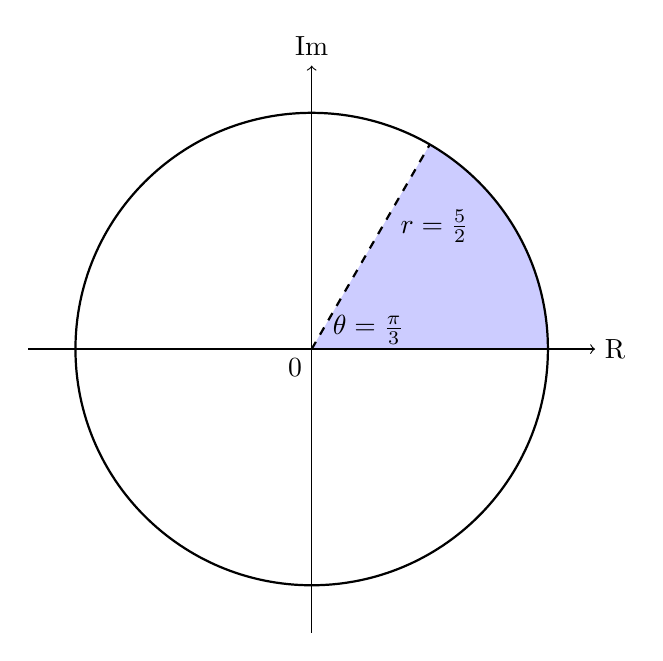
\begin{tikzpicture}[scale=1.2]
                \def\R{2.5}

                \draw[->] (-3,0) -- (3,0) node[right] {R};
                \draw[->] (0,-3) -- (0,3) node[above] {Im};


                \fill[blue!20]
                    (0,0) -- (\R,0) arc (0:60:\R) -- cycle;

                \draw[thick] (0,0) circle (\R);


                \draw[thick] (0,0) -- (\R,0);

                \draw[dashed, thick] (0,0) -- ({\R*cos(60)},{\R*sin(60)});

                \node at (0.6,0.2) {$\theta=\frac{\pi}{3}$};
                \node[below left] at (0,0) {$0$};
                \node at (1.3,1.3) {$r=\frac{5}{2}$};
            \end{tikzpicture}
        \end{center}
    \end{solution}


\end{document}